\section{Background}
The current models of the off-target problem in the CRISPR-Cas system can be divided into three types. Firstly, it can be modeled as purely "sequence alignment problem" similar to BLAST, which doesn't consider either the energy change or the experiment data; Secondly, it can be modeled with the help of experiment data; Thirdly, in a kinetic model, the energy change will be considered. 

Our model aims to investigate the off-target problem in the CRISPR-Cas system in an innovative kinetic model, therefore finding efficient ways to enhance the reliability of gene editing. Our motivation is based on our project Cell-free cancer detection. Firstly, there are no existing tools for evaluating sgRNA candidates' off-target probability with Cas13a, and the current tool for Cas12a is BLAST-based, which means that it is a rough model and can hardly take the case of single nucleotide mutation of cancer into account. The foundations of our model are mostly simple probability theory and energy theory, which make our model both convincing and pellucid.

\section{Introduction}
Currently, people have constructed a similar model as illustrated in the following figure \ref{fig:1}. There are four common rules when Cas nuclease cleaves the DNA\cite{klein2018hybridization}.
	.
\begin{figure}[tbph]
\centering
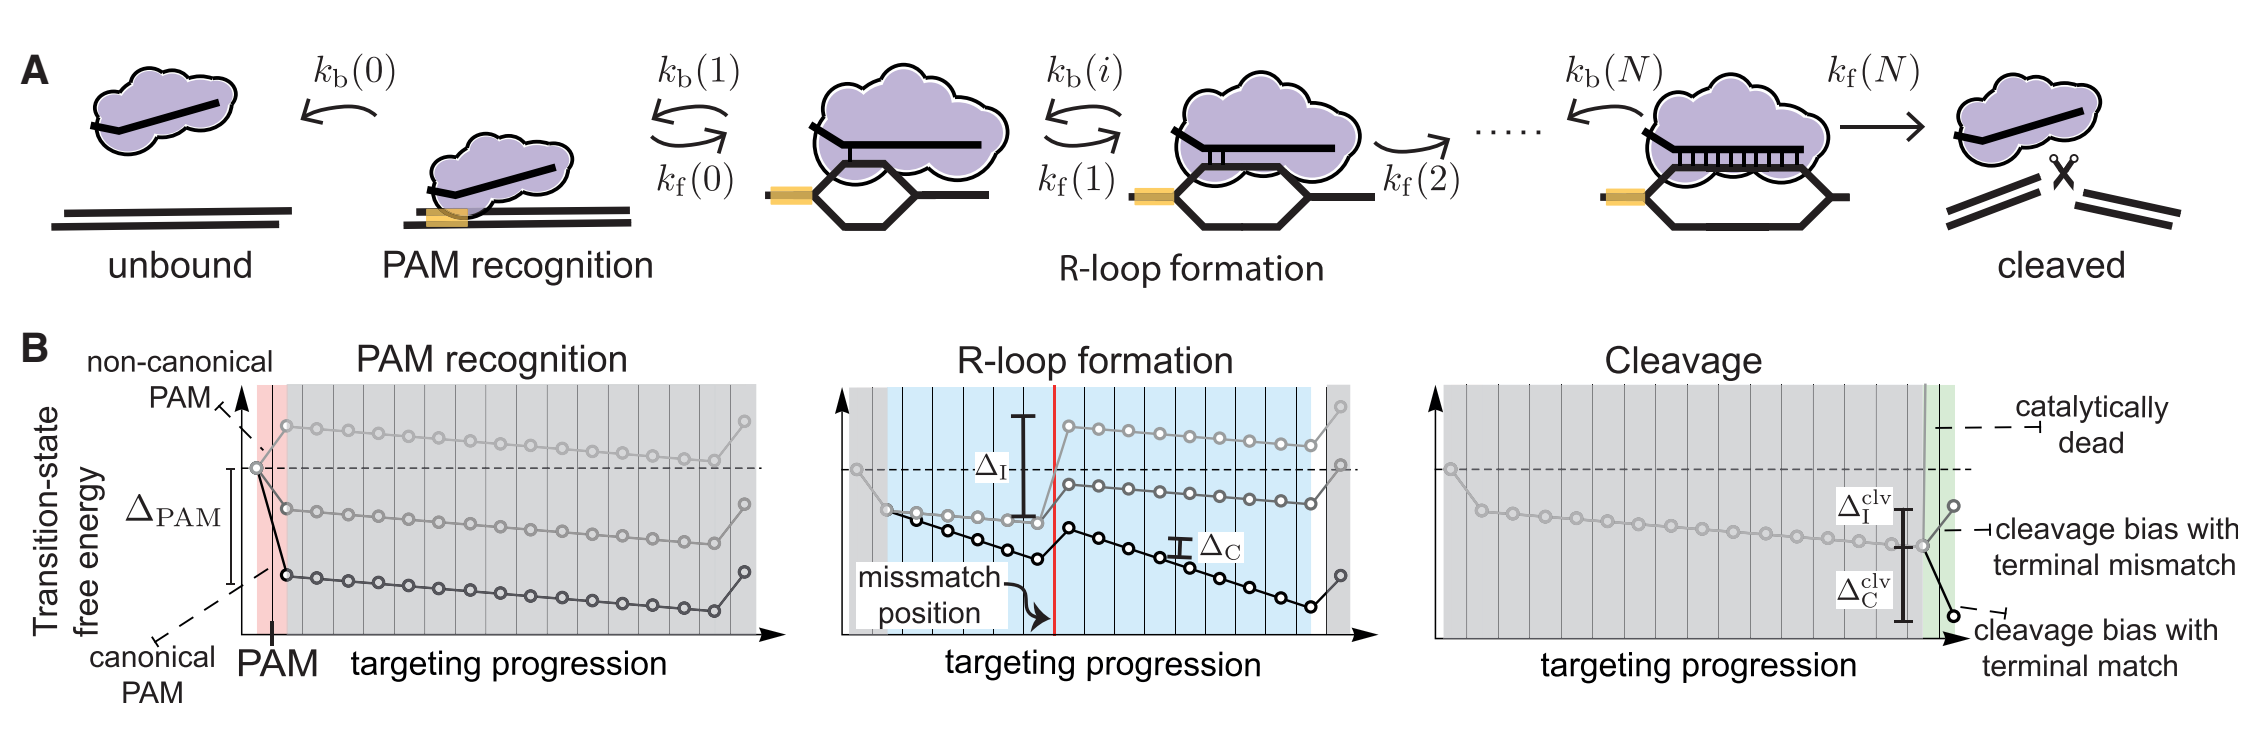
\includegraphics[width=3.5in]{1}
\caption{schematic diagram}
\label{fig:1}
\end{figure}
	
(1) Seed region: single mismatch(es) within a PAM proximal seed region can completely disrupt interference;\par
(2) Mismatch spread: when mismatches are outside the seed region, off-targets with spread out mismatches are targeted most strongly;\par
(3) Differential binding versus differential cleavage: binding is more tolerant of mismatches than cleavage;\par 
(4) Specificity-efficiency decoupling: weakened protein-DNA interactions can improve target selectivity while still maintaining efficiency;\par

Based on these four rules, probability theory is applied in to explain it. As we know, there are always only two results in an experiment, which are successful cleavage and unsuccessful cleavage. In math view, it can be one-hot encoded, and they are corresponding to 1 and 0. 

However, giving a 0/1 prediction is hard and unreliable. To solve this problem, one choice is to consider it as a cluster problem; however, it is easier to find a continuous quantitative function rather than to find a suitable cluster distance function. So naturally, finding an approximate probability distribution is a good choice. 
	
In many target design toolkits, they use a score function with several parameters which can generate a score to evaluate whether the target is good or bad. Here we consider the score function has the similar ability to probability, which is a description of "better" or "worse" while can’t affirm whether successful cleavage will appear. For our case, our goal is to find a function indicating which target is BETTER.
	
Considering the difference between model prediction and experimental data, our model consists of two aspects, which are kinetic inference and an updating module.